% =============================================================================
%  01-especificacao-tecnica.tex
%  Especificação técnica e memorial descritivo do esquemático "projeto_sabado"
%  (sequencial de 6 LEDs com NE555 + CD4017B) — compilar com pdflatex (2x)
% =============================================================================
\documentclass[11pt,a4paper]{article}
\usepackage[a4paper, left=2.2cm, right=2.2cm, top=2.4cm, bottom=2.3cm,
  headheight=14pt]{geometry}
\usepackage{projeto-sabado}
\usepackage{pdflscape}
\usepackage{fancyhdr}
\usepackage{titlesec}
\usepackage{lastpage}

% =============================================================================
%  figuras/esquematico.tex — redesenho do esquemático "projeto_sabado" (Rev. 01)
%  Netlist idêntica à do print do Altium, inclusive o resistor órfão R?
%  (mantido, isolado e marcado para remoção); só a disposição foi reorganizada
%  para leitura (sinal da esquerda para a direita, VCC em cima, GND embaixo).
%
%  Uso:  \esquematico          esquemático limpo
%        \esquematico[blocos]  com as molduras tracejadas dos blocos funcionais
%  Cores de rede (sempre com rótulo textual): VCC vermelho, clock petróleo,
%  reset dourado, saídas de LED oliva; demais em preto.
% =============================================================================
\newif\ifesqblocos
\newcommand{\esquematico}[1][]{%
\esqblocosfalse
\def\esqarg{#1}\def\esqblk{blocos}%
\ifx\esqarg\esqblk\esqblocostrue\fi
\begin{circuitikz}[american, line width=0.8pt, font=\fontepino]
\ctikzset{bipoles/length=1.25cm}

% ---------------------------------------------------------------- molduras
\ifesqblocos
  \draw[moldurabloco] (-0.35,4.55) rectangle (3.75,10.55);
  \node[titulobloco, anchor=south west] at (-0.25,4.6) {1 · ALIMENTAÇÃO};
  \draw[moldurabloco] (4.0,1.55) rectangle (11.95,10.55);
  \node[titulobloco, anchor=south west] at (4.1,1.6) {2 · OSCILADOR ASTÁVEL};
  \draw[moldurabloco] (12.1,1.55) rectangle (18.15,10.55);
  \node[titulobloco, anchor=south west] at (12.2,1.6) {3 · CONTADOR + 4 · RESET (Q6)};
  \draw[moldurabloco] (18.25,1.55) rectangle (23.45,11.15);
  \node[titulobloco, anchor=south west] at (18.35,1.6) {5 · INDICAÇÃO};
\fi

% ---------------------------------------------------------------- VCC
\draw[redeVcc] (2.85,11.0) -- (15.2,11.0);
\node[rede, text=redeVcc, anchor=south west] at (2.9,11.0) {VCC};

% ---------------------------------------------------------------- 1 · ALIMENTAÇÃO
\fonteVcima[{\begin{tabular}{@{}l@{}}CR2032 · 3 V\textsuperscript{\,inf.}\\[-1pt]\scriptsize BAT-HLD-001\\[-2pt]\scriptsize (duas abas +)\end{tabular}}]{1.0}{6.3}{8.5}{\textsf{BT1}}
\draw (1.0,6.3) -- (1.0,5.6) node[ground]{};
\draw (1.0,8.5) -- (1.0,10.0) -- (1.5,10.0) node[spdt, anchor=in] (SW) {};
\node[rede, left] at (1.0,9.3) {BAT+};
\draw[redeVcc] (SW.out 1) -| (2.85,11.0);
\draw (SW.out 2) -- ++(0.35,0) coordinate (swnc);
\marcaNC{swnc}
\node[font=\fontenum, above left, inner sep=1pt] at (SW.in) {1};
\node[font=\fontenum, above, inner sep=1pt] at ($(SW.out 1)+(0.15,0)$) {2};
\node[font=\fontenum, below, inner sep=1.5pt] at (SW.out 2) {3};
\node[font=\fontepino\bfseries, anchor=north] at ($(SW.out 2)+(-0.1,-0.3)$) {SW1};
\node[font=\scriptsize\sffamily, anchor=north, text=charcoal, align=center]
  at ($(SW.out 2)+(-0.1,-0.65)$) {PCM12SMTR\\[-1pt]pinos 4–7 (MNT):\\[-1pt]sem ligação};

% ---------------------------------------------------------------- 2 · OSCILADOR (U1)
\draw[ci] (7.0,4.6) rectangle (10.0,8.6);
\pinoC{7.6}{8.6}{8}{VCC}{u1p8}
\pinoC{9.4}{8.6}{4}{$\overline{\textsf{RESET}}$}{u1p4}
\pinoE{7.0}{7.8}{7}{DISCH}{u1p7}
\pinoE{7.0}{6.6}{6}{THRES}{u1p6}
\pinoE{7.0}{5.4}{2}{TRIG}{u1p2}
\pinoD{10.0}{6.6}{3}{OUT}{u1p3}
\pinoB{7.6}{4.6}{1}{GND}{u1p1}
\pinoB{9.4}{4.6}{5}{CONT}{u1p5}
\node[align=center, font=\fontepino] at (8.75,7.35) {\textbf{U1}\\NE555DR};
% alimentação do 555 (RESET amarrado ao VCC)
\draw[redeVcc] (u1p8) -- (7.6,11.0);
\draw[redeVcc] (u1p4) -- (9.4,11.0);
\fill[redeVcc] (7.6,11.0) circle (2.2pt) (9.4,11.0) circle (2.2pt);
% rede de temporização R1-R2-C2
\draw (5.0,11.0) to[R, l_={$R_1$}, a^={\SI{1.2}{\kilo\ohm}}] (5.0,7.8);
\fill[redeVcc] (5.0,11.0) circle (2.2pt);
\draw (5.0,7.8) to[R, l_={$R_2$}, a^={\SI{10}{\kilo\ohm}}] (5.0,6.0);
\draw (5.0,6.0) to[C, l_={$C_2$}, a^={\SI{10}{\micro\farad}}] (5.0,2.8) node[ground]{};
\draw (5.0,7.8) -- (u1p7);
\draw (5.0,6.0) -- (6.0,6.0);
\draw (u1p6) -- (6.0,6.6) -- (6.0,5.4) -- (u1p2);
\node[circ] at (5.0,7.8) {};
\node[circ] at (5.0,6.0) {};
\node[circ] at (6.0,6.0) {};
\node[rede, above] at (5.75,7.8) {DIS};
\node[rede, below] at (5.5,6.0) {THR};
% GND e CONT
\draw (u1p1) -- (7.6,2.8) node[ground]{};
\draw (u1p5) to[C, l_={$C_1$}, a^={\SI{10}{\nano\farad}}] (9.4,2.8) node[ground]{};
\node[rede, right] at (9.45,3.85) {CV};

% saída do 555 -> clock do 4017 (porta OUT555 do original)
\draw[petroleo, line width=1pt] (u1p3) -- (11.8,6.6) -- (11.8,8.6) -- (13.0,8.6);
\node[rede, text=petroleo, above=1.5pt] at (11.2,6.6) {OUT555};

% ---------------------------------------------------------------- 3 · CONTADOR (U2)
\draw[ci] (13.6,3.4) rectangle (16.8,9.6);
\pinoC{15.2}{9.6}{16}{VDD}{u2p16}
\pinoE{13.6}{8.6}{14}{\hspace{2.2mm}CLK}{u2p14}
\draw[line width=0.7pt] (13.6,8.75) -- (13.82,8.6) -- (13.6,8.45);
\pinoE{13.6}{7.6}{13}{CLK INH}{u2p13}
\pinoE{13.6}{4.4}{8}{VSS}{u2p8}
\pinoB{16.0}{3.4}{15}{RESET}{u2p15}
\pinoD{16.8}{9.2}{3}{Q0}{u2q0}
\pinoD{16.8}{8.7}{2}{Q1}{u2q1}
\pinoD{16.8}{8.2}{4}{Q2}{u2q2}
\pinoD{16.8}{7.7}{7}{Q3}{u2q3}
\pinoD{16.8}{7.2}{10}{Q4}{u2q4}
\pinoD{16.8}{6.7}{1}{Q5}{u2q5}
\pinoD{16.8}{6.2}{5}{Q6}{u2q6}
\pinoD{16.8}{5.7}{6}{Q7}{u2q7}
\pinoD{16.8}{5.2}{9}{Q8}{u2q8}
\pinoD{16.8}{4.7}{11}{Q9}{u2q9}
\pinoD{16.8}{4.2}{12}{CO}{u2co}
\marcaNC{u2q7}\marcaNC{u2q8}\marcaNC{u2q9}\marcaNC{u2co}
\node[align=center, font=\fontepino] at (15.15,6.0) {\textbf{U2}\\CD4017BM96};
\draw[redeVcc] (u2p16) -- (15.2,11.0);
\draw (u2p13) -- (12.65,7.6) -- (12.65,7.0) node[ground]{};
\draw (u2p8) -- (12.65,4.4) -- (12.65,3.8) node[ground]{};

% ---------------------------------------------------------------- 4 · REALIMENTAÇÃO Q6 -> RESET
\draw[douradoEsc, line width=1pt] (u2q6) -- (17.9,6.2) -- (17.9,2.3) -- (16.0,2.3) -- (u2p15);
\node[rede, text=douradoEsc, above=2pt] at (16.85,2.3) {Q6 → RESET};

% ---------------------------------------------------------------- 5 · INDICAÇÃO (D1..D6, R3)
\foreach \q/\xj/\yl/\d in {u2q0/18.4/10.45/1, u2q1/18.9/9.45/2, u2q2/19.4/8.45/3,
                           u2q3/19.4/7.45/4, u2q4/18.9/6.45/5, u2q5/18.4/5.45/6}{
  \draw[oliva, line width=0.9pt] (\q) -| (\xj,\yl) -- (20.2,\yl);
  \draw (20.2,\yl) to[led] (21.6,\yl) -- (22.2,\yl);
  \node[font=\fontepino, anchor=south east, inner sep=1pt] at (20.15,\yl+0.04) {D\d};
}
\draw (22.2,10.45) -- (22.2,4.6) to[R, l_={$R_3$}, a^={\SI{120}{\ohm}}] (22.2,3.0) node[ground]{};
\foreach \yl in {9.45,8.45,7.45,6.45,5.45}{\node[circ] at (22.2,\yl) {};}
\node[font=\footnotesize\sffamily, text=charcoal, align=center, anchor=north]
  at (20.55,4.95) {LED verde 0805 (×6)\\[-1pt]anodo (pino 2) à esquerda};
\node[rede, right=2.5pt] at (22.2,4.85) {LED\_K};

% ---------------------------------------------------------------- resíduo do original
% resistor RES_0805C sem designador e sem ligação, como no print (deve ser apagado)
\draw (0.6,3.95) to[R] (0.6,2.35);
\marcaNC{0.6,3.95}\marcaNC{0.6,2.35}
\node[font=\fontepino, anchor=west] at (1.0,3.35) {R? (RES\_0805C)};
\node[font=\scriptsize\sffamily, anchor=west, text=redeVcc] at (1.0,2.9) {solto, sem designador:};
\node[font=\scriptsize\sffamily, anchor=west, text=redeVcc] at (1.0,2.55) {remover};
\end{circuitikz}%
}

% =============================================================================
%  figuras/blocos.tex — diagrama de blocos funcional do sequencial de LEDs
%  \diagramaBlocos                         todos os blocos em pé de igualdade
%  \diagramaBlocos[b3/.style={destaque}]   destaca o bloco 3 (usado no tutorial)
%  \diagramaBlocos[todosapagados, b2/.style={destaque}] apaga os demais
% =============================================================================
\tikzset{
  b1/.style={}, b2/.style={}, b3/.style={}, b4/.style={}, b5/.style={},
  blocofunc/.style={draw=charcoal, line width=0.8pt, rounded corners=2mm,
    fill=white, align=center, font=\footnotesize\sffamily, text width=2.75cm,
    minimum height=2.0cm, inner sep=3pt},
  destaque/.style={fill=petroleo, draw=petroleo, text=white, line width=1.3pt},
  apagado/.style={draw=charcoal!35, text=charcoal!45},
  todosapagados/.style={blocofunc/.append style={apagado}},
  sinal/.style={-{Latex[length=2.4mm]}, line width=0.95pt, draw=charcoal},
  energia/.style={dashed, line width=0.9pt, draw=redeVcc},
  rotsinal/.style={font=\footnotesize\sffamily, align=center, inner sep=1.5pt},
}
\newcommand{\diagramaBlocos}[1][]{%
\begin{tikzpicture}[#1]
  \node[blocofunc, b1] (b1) at (0,0)
    {\textbf{1 · Alimentação}\\BT1 (CR2032)\\SW1 liga/desliga};
  \node[blocofunc, b2] (b2) at (4.5,0)
    {\textbf{2 · Oscilador}\\U1 NE555\\astável\\$f\approx\SI{6,8}{\hertz}$};
  \node[blocofunc, b3] (b3) at (9.0,0)
    {\textbf{3 · Contador}\\U2 CD4017B\\Johnson +\\decodificador};
  \node[blocofunc, b5] (b5) at (13.5,0)
    {\textbf{5 · Indicação}\\D1–D6 + R3\\um LED aceso\\por vez};
  \node[blocofunc, b4, minimum height=1.25cm, text width=3.9cm] (b4) at (9.0,-2.75)
    {\textbf{4 · Realimentação}\\Q6 $\rightarrow$ RESET (módulo 6)};
  % ---------------- energia (tracejado): VCC distribuído a U1 e U2
  \draw[energia] (b1.north) -- ++(0,0.55) coordinate (e0) -- (e0 -| b3.north);
  \draw[energia, -{Latex[length=2mm]}] (e0 -| b2.north) -- (b2.north);
  \draw[energia, -{Latex[length=2mm]}] (e0 -| b3.north) -- (b3.north);
  \node[rotsinal, text=redeVcc, above] at ($(e0)!0.5!(e0 -| b2.north)$) {VCC $\approx$ \SI{3}{\volt}};
  % ---------------- sinais
  \draw[sinal] (b2) -- node[rotsinal, above] {CLK} node[rotsinal, below] {OUT555} (b3);
  \draw[sinal] (b3) -- node[rotsinal, above] {Q0…Q5} node[rotsinal, below] {1 de 6} (b5);
  \draw[sinal] ([xshift=7mm]b3.south) -- node[rotsinal, right] {Q6} ([xshift=7mm]b4.north);
  \draw[sinal] ([xshift=-7mm]b4.north) -- node[rotsinal, left] {RESET} ([xshift=-7mm]b3.south);
\end{tikzpicture}}

% =============================================================================
%  figuras/ne555-interno.tex — modelo funcional interno do 555 (didático)
%  Divisor de três resistores iguais, dois comparadores, flip-flop S-R,
%  estágio de saída e transistor de descarga. Pinos com a ligação externa
%  usada no projeto_sabado.
% =============================================================================
\newcommand{\neInterno}{%
\begin{circuitikz}[american, line width=0.8pt, font=\fontepino]
\ctikzset{bipoles/length=0.95cm}
% contorno do CI
\draw[ci, rounded corners=1.5mm, fill=douradoClaro!60] (3.0,0.4) rectangle (11.2,8.6);
\node[font=\fontepino\bfseries, anchor=south west, text=charcoal] at (6.2,0.5) {NE555 (U1)};
% pinos
\draw (3.8,8.6) -- (3.8,9.2) node[above, font=\fontepino, align=center] {8 VCC\\[-1pt]\scriptsize alimentação};
\draw (5.4,8.6) -- (5.4,9.2) node[above, font=\fontepino, align=center] {6 THRES\\[-1pt]\scriptsize ← nó THR};
\draw (8.3,8.6) -- (8.3,9.2) node[above, font=\fontepino, align=center] {4 $\overline{\textsf{RESET}}$\\[-1pt]\scriptsize ← VCC};
\draw (3.8,0.4) -- (3.8,-0.2) node[below, font=\fontepino, align=center] {1 GND\\[-1pt]\scriptsize referência};
\draw (5.4,0.4) -- (5.4,-0.2) node[below, font=\fontepino, align=center] {2 TRIG\\[-1pt]\scriptsize ← nó THR};
\draw (3.0,5.6) -- (2.4,5.6) node[left, font=\fontepino, align=right] {5 CONT\\[-1pt]\scriptsize → C1 → GND};
\draw (11.2,6.1) -- (11.8,6.1) node[right, font=\fontepino, align=left] {3 OUT\\[-1pt]\scriptsize → CLK de U2};
\draw (11.2,2.8) -- (11.8,2.8) node[right, font=\fontepino, align=left] {7 DISCH\\[-1pt]\scriptsize ← nó DIS};
% divisor interno
\draw (3.8,8.6) to[R, l_={$R$}] (3.8,5.6) to[R, l_={$R$}] (3.8,3.0) to[R, l_={$R$}] (3.8,0.4);
\node[circ] at (3.8,5.6) {};
\node[circ] at (3.8,3.0) {};
\node[font=\scriptsize\sffamily, anchor=south] at (4.45,5.62) {$2V_{CC}/3$};
\node[font=\scriptsize\sffamily, anchor=south] at (4.45,3.02) {$V_{CC}/3$};
% comparador A (limiar): + = THRES, - = 2/3 VCC
\node[op amp, noinv input up, scale=0.8] (cA) at (6.6,6.1) {};
\draw (5.4,8.6) |- (cA.+);
\draw (3.8,5.6) -| ($(cA.-)+(-0.35,0)$) -- (cA.-);
\node[font=\footnotesize\sffamily, above, text=charcoal] at (6.7,6.75) {comp. A (limiar)};
% comparador B (disparo): + = 1/3 VCC, - = TRIG
\node[op amp, noinv input up, scale=0.8] (cB) at (6.6,2.5) {};
\draw (3.8,3.0) -| ($(cB.+)+(-0.35,0)$) -- (cB.+);
\draw (5.4,0.4) |- (cB.-);
\node[font=\footnotesize\sffamily, below, text=charcoal] at (6.7,1.85) {comp. B (disparo)};
% flip-flop S-R
\draw[line width=0.9pt, fill=white] (8.0,1.9) rectangle (9.3,6.7);
\node[font=\fontepino\bfseries, rotate=90] at (8.65,4.3) {flip-flop S-R};
\draw (cA.out) -- (8.0,6.1);  \node[font=\scriptsize\sffamily, right] at (8.0,6.1) {R};
\draw (cB.out) -- (8.0,2.5);  \node[font=\scriptsize\sffamily, right] at (8.0,2.5) {S};
\node[font=\scriptsize\sffamily, left] at (9.3,6.1) {$Q$};
\node[font=\scriptsize\sffamily, left] at (9.3,2.5) {$\overline{Q}$};
\draw (8.3,8.6) -- (8.3,6.85);
\draw[fill=white] (8.3,6.78) circle (0.08);
% estágio de saída (buffer)
\draw (9.3,6.1) -- (9.7,6.1);
\draw[line width=0.9pt, fill=white] (9.7,5.75) -- (9.7,6.45) -- (10.45,6.1) -- cycle;
\draw (10.45,6.1) -- (11.2,6.1);
\node[font=\footnotesize\sffamily, above, text=charcoal] at (10.05,6.45) {saída};
% transistor de descarga
\node[npn, scale=0.85] (Qd) at (10.2,1.75) {};
\draw (9.3,2.5) -- (9.55,2.5) |- (Qd.B);
\draw (Qd.C) |- (11.2,2.8);
\draw (Qd.E) -- ++(0,-0.15) node[ground, scale=0.8]{};
\node[font=\footnotesize\sffamily, anchor=east, text=charcoal] at (9.45,1.0) {descarga};
\end{circuitikz}}

% =============================================================================
%  figuras/cd4017-interno.tex — modelo funcional do CD4017B (didático)
%  Condicionamento de clock (Schmitt) -> contador Johnson de 5 estágios
%  (realimentação pelo complemento do último estágio) -> decodificador 1-de-10.
%  Modelo lógico equivalente; a implementação interna do fabricante pode
%  usar portas diferentes com o mesmo comportamento externo.
% =============================================================================
\tikzset{
  ffj/.style={draw=charcoal, line width=0.8pt, fill=white, minimum width=0.95cm,
    minimum height=1.05cm, font=\footnotesize\sffamily, align=center, inner sep=1pt},
  blk/.style={draw=charcoal, line width=0.9pt, fill=white, rounded corners=1.5mm,
    align=center, font=\footnotesize\sffamily, inner sep=3pt},
  fio/.style={-{Latex[length=2mm]}, line width=0.8pt},
}
\newcommand{\cdInterno}{%
\begin{tikzpicture}[font=\fontepino]
  % contorno do CI
  \draw[ci, rounded corners=1.5mm, fill=douradoClaro!60] (-0.4,-1.15) rectangle (12.5,3.35);
  \node[font=\fontepino\bfseries, anchor=north west, text=charcoal] at (-0.3,3.3) {CD4017B (U2)};
  % condicionamento do clock
  \node[blk, text width=2.1cm, minimum height=1.6cm] (cond) at (0.85,1.2)
    {Schmitt-trigger\\+ habilitação\\[1pt]\scriptsize avança na borda $\uparrow$ se INH = 0};
  \draw[fio] (-1.4,1.65) node[left, font=\fontepino, align=right] {14 CLK\\[-1pt]\scriptsize ← OUT555} -- (cond.west |- 0,1.65);
  \draw[fio] (-1.4,0.75) node[left, font=\fontepino, align=right] {13 CLK INH\\[-1pt]\scriptsize ← GND} -- (cond.west |- 0,0.75);
  % contador Johnson de 5 estágios
  \draw[line width=0.8pt, rounded corners=1.5mm, draw=petroleo, fill=petroleoClaro]
    (2.55,-0.25) rectangle (9.35,2.95);
  \node[font=\scriptsize\sffamily\bfseries, text=petroleo, anchor=north west] at (2.6,2.92)
    {contador Johnson de 5 estágios};
  \foreach \n/\x in {A/3.55, B/4.85, C/6.15, D/7.45, E/8.75}{
    \node[ffj] (ff\n) at (\x,1.2) {FF \n\\[-1pt]D\enspace Q};
  }
  \foreach \a/\b in {A/B, B/C, C/D, D/E}{\draw[fio] (ff\a.east) -- (ff\b.west);}
  % realimentação: complemento do estágio E volta para o D de A
  \draw[fio, douradoEsc] (ffE.north) -- ++(0,0.55) -| ($(ffA.west)+(-0.35,0)$) -- (ffA.west);
  \node[font=\scriptsize\sffamily, text=douradoEsc, above] at (7.6,2.3) {$\overline{E}\rightarrow D_A$};
  % clock interno para todos os estágios
  \draw[fio] (cond.east |- 0,0.2) -- (2.95,0.2);
  \draw[line width=0.6pt, dashed] (2.95,0.2) -- (8.75,0.2);
  \foreach \x in {3.55,4.85,6.15,7.45,8.75}{\draw[-{Latex[length=1.5mm]}, line width=0.6pt] (\x,0.2) -- (\x,0.67);}
  \node[font=\footnotesize\sffamily, below] at (5.6,0.18) {clock interno (todos os estágios)};
  % reset assíncrono
  \draw[fio, douradoEsc] (5.1,-1.9) node[below, font=\fontepino, align=center] {15 RESET ← Q6 (pino 5)\\[-1pt]\scriptsize assíncrono: força a contagem 0} -- (5.1,-0.25);
  % decodificador
  \node[blk, text width=1.75cm, minimum height=3.1cm] (dec) at (11.25,1.35)
    {decodificador\\1-de-10\\[2pt]\scriptsize 10 portas\\AND de 2\\entradas};
  \draw[line width=2.2pt, -{Latex[length=2.6mm, width=3.2mm]}] (9.35,1.2) -- node[above=2pt, font=\footnotesize\sffamily] {A…E} (dec.west |- 0,1.2);
  % saídas
  \foreach \q/\p/\y in {0/3/2.55, 1/2/2.1, 2/4/1.65, 3/7/1.2, 4/10/0.75, 5/1/0.3, 6/5/-0.15}{
    \draw[fio, oliva] (dec.east |- 0,\y) -- (12.9,\y);
    \node[font=\scriptsize\sffamily, right] at (12.9,\y) {Q\q\ (\p)};
  }
  \node[font=\scriptsize\sffamily, right, align=left, text=charcoal] at (12.9,-0.75)
    {Q7 (6), Q8 (9),\\Q9 (11): sem uso};
  % carry-out
  \draw[fio, charcoal] (8.75,-0.25) -- (8.75,-1.9) node[below, font=\fontepino, align=center] {12 CO $=\overline{E}$\\[-1pt]\scriptsize sem uso};
\end{tikzpicture}}

% =============================================================================
%  figuras/pinagem.tex — pinagem ilustrada dos CIs (vista superior, SOIC)
%  Proporções do encapsulamento SOIC (JEDEC MS-012): corpo 3,9 mm de largura,
%  passo 1,27 mm; comprimento 4,9 mm (8 pinos) e 9,9 mm (16 pinos).
%  Escala do desenho: 0,75 cm por mm (≈ 7,5:1). Cor do terminal = rede.
% =============================================================================
\def\pgS{0.75}
\pgfmathsetmacro{\pgP}{1.27*\pgS}     % passo
\pgfmathsetmacro{\pgBW}{1.95*\pgS}    % meia largura do corpo
\pgfmathsetmacro{\pgLL}{1.05*\pgS}    % comprimento do terminal fora do corpo
\pgfmathsetmacro{\pgLH}{0.205*\pgS}   % meia largura do terminal
% \terminalE{y}{num}{nome}{rede}{cor}  terminal do lado esquerdo
\newcommand{\terminalE}[5]{%
  \fill[#5] ({-\pgBW-\pgLL},{#1-\pgLH}) rectangle ({-\pgBW},{#1+\pgLH});
  \draw[line width=0.4pt, charcoal] ({-\pgBW-\pgLL},{#1-\pgLH}) rectangle ({-\pgBW},{#1+\pgLH});
  \node[font=\footnotesize\sffamily\bfseries, anchor=east] at ({-\pgBW-\pgLL-0.08},#1) {#2};
  \node[font=\footnotesize\sffamily, anchor=east] at ({-\pgBW-\pgLL-0.5},#1) {#3};
  \node[font=\scriptsize\sffamily, anchor=east, text=#5] at ({-\pgBW-\pgLL-2.35},#1) {#4};}
% \terminalD{y}{num}{nome}{rede}{cor}  terminal do lado direito
\newcommand{\terminalD}[5]{%
  \fill[#5] ({\pgBW},{#1-\pgLH}) rectangle ({\pgBW+\pgLL},{#1+\pgLH});
  \draw[line width=0.4pt, charcoal] ({\pgBW},{#1-\pgLH}) rectangle ({\pgBW+\pgLL},{#1+\pgLH});
  \node[font=\footnotesize\sffamily\bfseries, anchor=west] at ({\pgBW+\pgLL+0.08},#1) {#2};
  \node[font=\footnotesize\sffamily, anchor=west] at ({\pgBW+\pgLL+0.5},#1) {#3};
  \node[font=\scriptsize\sffamily, anchor=west, text=#5] at ({\pgBW+\pgLL+2.35},#1) {#4};}
% corpo SOIC: \corpoSOIC{meio comprimento em mm}{marcação}{subtítulo}
\newcommand{\corpoSOIC}[3]{%
  \pgfmathsetmacro{\pgBL}{#1*\pgS}%
  \fill[rounded corners=1mm, fill=charcoal!95!black] ({-\pgBW},{-\pgBL}) rectangle ({\pgBW},{\pgBL});
  \fill[gray!55] ({-\pgBW+0.38},{\pgBL-0.38}) circle (0.13);
  \node[text=white, font=\small\sffamily\bfseries, rotate=90] at (0,0.15) {#2};
  \node[text=white!80!gray, font=\scriptsize\sffamily, rotate=90] at (0.55,0.15) {#3};}

% ------------------------------------------------------------------ NE555DR
\newcommand{\pinagemNE}{%
\begin{tikzpicture}
  \corpoSOIC{2.45}{NE555}{D (SOIC-8) · TI}
  \pgfmathsetmacro{\yA}{1.5*\pgP}\pgfmathsetmacro{\yB}{0.5*\pgP}
  \pgfmathsetmacro{\yC}{-0.5*\pgP}\pgfmathsetmacro{\yD}{-1.5*\pgP}
  \terminalE{\yA}{1}{GND}{GND}{charcoal}
  \terminalE{\yB}{2}{TRIG}{THR (C2, R2)}{black}
  \terminalE{\yC}{3}{OUT}{OUT555 → U2.14}{petroleo}
  \terminalE{\yD}{4}{$\overline{\textsf{RESET}}$}{VCC}{redeVcc}
  \terminalD{\yA}{8}{VCC}{VCC}{redeVcc}
  \terminalD{\yB}{7}{DISCH}{DIS (R1, R2)}{black}
  \terminalD{\yC}{6}{THRES}{THR (C2, R2)}{black}
  \terminalD{\yD}{5}{CONT}{CV (C1 → GND)}{black}
  \node[font=\footnotesize\sffamily\bfseries, anchor=south] at (0,2.25) {U1 — NE555DR};
\end{tikzpicture}}

% ------------------------------------------------------------------ CD4017BM96
\newcommand{\pinagemCD}{%
\begin{tikzpicture}
  \corpoSOIC{4.95}{CD4017B}{D/M (SOIC-16) · TI}
  \foreach \i/\n/\nome/\rede/\cor in {
      1/1/Q5/{→ D6}/oliva, 2/2/Q1/{→ D2}/oliva, 3/3/Q0/{→ D1}/oliva,
      4/4/Q2/{→ D3}/oliva, 5/5/Q6/{→ RESET (15)}/douradoEsc, 6/6/Q7/{sem uso}/cinzaNC,
      7/7/Q3/{→ D4}/oliva, 8/8/VSS/{GND}/charcoal}{
    \pgfmathsetmacro{\yy}{(4.5-\i)*\pgP}
    \terminalE{\yy}{\n}{\nome}{\rede}{\cor}
  }
  \foreach \i/\n/\nome/\rede/\cor in {
      1/16/VDD/{VCC}/redeVcc, 2/15/RESET/{← Q6 (5)}/douradoEsc,
      3/14/CLK/{← OUT555 (U1.3)}/petroleo, 4/13/CLK INH/{GND}/charcoal,
      5/12/CO/{sem uso}/cinzaNC, 6/11/Q9/{sem uso}/cinzaNC,
      7/10/Q4/{→ D5}/oliva, 8/9/Q8/{sem uso}/cinzaNC}{
    \pgfmathsetmacro{\yy}{(4.5-\i)*\pgP}
    \terminalD{\yy}{\n}{\nome}{\rede}{\cor}
  }
  \node[font=\footnotesize\sffamily\bfseries, anchor=south] at (0,4.0) {U2 — CD4017BM96};
\end{tikzpicture}}

% ------------------------------------------------------------------ legenda de cores
\newcommand{\legendaRedes}{%
\begin{tikzpicture}[font=\scriptsize\sffamily]
  \foreach \cor/\txt/\x in {redeVcc/VCC/0, charcoal/GND/1.45, petroleo/clock (OUT555)/2.9,
                           douradoEsc/reset (Q6)/5.85, oliva/saídas de LED/8.3,
                           black/temporização/11.0, cinzaNC/sem uso/13.6}{
    \fill[\cor] (\x,-0.12) rectangle ++(0.42,0.24);
    \node[anchor=west] at (\x+0.48,0) {\txt};
  }
\end{tikzpicture}}

% =============================================================================
%  referencias.tex — fontes verificadas (datasheets lidos nos PDFs oficiais
%  em 20–21/11/2026) e trechos de especificação reutilizados no texto.
% =============================================================================

% ---------------------------------------------------------------- trechos
\newcommand{\DSbat}{tensão nominal de \SI{3}{\volt} e corte em \SI{2}{\volt};
capacidade de \SI{225}{\milli\ampere\hour} (Panasonic) a \SI{254}{\milli\ampere\hour}
(Energizer, carga de \SI{15}{\kilo\ohm} até \SI{2}{\volt}, \SI{21}{\celsius}). Essa
capacidade é especificada com dreno contínuo de cerca de \SI{0,2}{\milli\ampere}; a
resistência interna da célula nova fica perto de \SI{10}{\ohm}~\cite{cr2032pan,cr2032en,enerman}.}

\newcommand{\DSsuporte}{o suporte faz o contato positivo pelo próprio corpo metálico,
soldado em quatro ilhas laterais (duas de cada lado, no footprint recomendado); o
negativo é uma \textbf{ilha circular de cobre de \SI{18}{\milli\meter} de diâmetro na
própria placa}, sob a bateria, que precisa ficar exposta e ligada ao GND. O desenho do
fabricante é para CR2032 (o catálogo também lista a CR2025)~\cite{bathld}.}

\newcommand{\DSsw}{SPDT, \SI{300}{\milli\ampere} a \SI{6}{\volt} CC, vida mecânica de
\num{10000} ciclos e operação de \SIrange{-20}{85}{\celsius}, segundo distribuidores. O
PDF do fabricante (C\&K, hoje Littelfuse) não pôde ser lido na verificação; por isso o
terminal comum e o significado do sufixo SMTR ficam sem confirmação. A DigiKey marca a
peça como obsoleta~\cite{pcm12}.}

\newcommand{\DSneEnc}{SOIC-8 (sufixo D); o R final indica carretel de 2500 unidades. A
versão em tubo (NE555D) consta como obsoleta~\cite{ne555}.}

\newcommand{\DSne}{VCC recomendada de \SIrange{4,5}{16}{\volt}; consumo sem carga a
\SI{5}{\volt} de \SI{3}{\milli\ampere} típicos e \SI{6}{\milli\ampere} máximos com a saída
baixa (\SI{2}{\milli\ampere} e \SI{5}{\milli\ampere} com a saída alta); limiares de cerca de
$2V_{CC}/3$ (THRES) e $V_{CC}/3$ (TRIG); RESET ativo abaixo de 0,3 a \SI{1}{\volt}, e o
datasheet manda ligá-lo ao VCC quando não usado; saída de até \SI{200}{\milli\ampere};
\SI{0,01}{\micro\farad} no CONT no circuito astável de referência; desacoplamento do VCC
com cerâmico de \SI{0,1}{\micro\farad}; operação de \SIrange{0}{70}{\celsius}~\cite{ne555}.}

\newcommand{\DScdEnc}{SOIC-16 (sufixo M); o 96 indica carretel de 2500 unidades. A
versão em tubo (CD4017BM) consta como obsoleta~\cite{cd4017}.}

\newcommand{\DScd}{VDD recomendada de \SIrange{3}{18}{\volt}; avança na borda de subida
do CLOCK com CLOCK INHIBIT em nível baixo; gatilho Schmitt na entrada de clock, que aceita
bordas lentas; RESET ativo em nível alto, que leva a contagem a zero. A \SI{5}{\volt}:
clock máximo de \SI{2,5}{\mega\hertz} (mín.) e \SI{5}{\mega\hertz} (típ.), atraso
RESET\,$\to$\,saída de \SI{265}{\nano\second} típicos e \SI{530}{\nano\second} máximos,
largura mínima recomendada do pulso de reset de \SI{260}{\nano\second} e corrente
quiescente máxima de \SI{5}{\micro\ampere} a \SI{25}{\celsius}. O datasheet não tem
tabelas a \SI{3}{\volt}, só a 5, 10 e \SI{15}{\volt}~\cite{cd4017}.}

\newcommand{\DScap}{Exemplo de código: Murata GRM21BR61A106KE19 (\SI{10}{\micro\farad}
$\pm$\SI{10}{\percent}, X5R, \SI{10}{\volt})~\cite{murata}. A perda de capacitância com
tensão contínua aplicada varia de modelo para modelo e deve ser lida na curva do
fabricante.}

\newcommand{\DSres}{exemplo: Yageo série RC, RC0805 com \SI{0,125}{\watt} a
\SI{70}{\celsius} e \SI{150}{\volt} de tensão máxima de trabalho~\cite{yageo}.}

\newcommand{\DSled}{Dois LEDs 0805 do mesmo fabricante mostram a diferença que importa:
o Kingbright APT2012SGC (GaP, \SI{568}{\nano\meter}) tem Vf de \SI{2,2}{\volt} típicos e
\SI{2,5}{\volt} máximos a \SI{20}{\milli\ampere}; o APT2012ZGC (InGaN, \SI{525}{\nano\meter})
tem \SI{3,3}{\volt} típicos e \SI{4,1}{\volt} máximos. Os dois admitem \SI{25}{\milli\ampere}
contínuos~\cite{kingbright}.}

\newcommand{\DSneVcc}{\SIrange{4,5}{16}{\volt}~\cite{ne555}}
\newcommand{\DScdVdd}{\SIrange{3}{18}{\volt}~\cite{cd4017}}
\newcommand{\DSswI}{\SI{300}{\milli\ampere} a \SI{6}{\volt} CC (distribuidor)~\cite{pcm12}}
\newcommand{\DSbatI}{Capacidade especificada com dreno de $\approx$\SI{0,2}{\milli\ampere}; dreno alto reduz a capacidade útil~\cite{cr2032en,enerman}}
\newcommand{\DScmos}{LMC555: opera a partir de \SI{1,5}{\volt}; TLC555C: a partir de
\SI{2}{\volt} (a versão TLC555I só a partir de \SI{3}{\volt}); os dois consomem cerca de
\SI{180}{\micro\ampere} típicos a \SI{5}{\volt} e são pino a pino com o 555~\cite{lmc555,tlc555}}
\newcommand{\DSledcomp}{APT2012SGC $\times$ APT2012ZGC~\cite{kingbright}}
\newcommand{\DSaltium}{\cite{altium}}

% ---------------------------------------------------------------- lista
\newcommand{\listaReferencias}{%
\begingroup
\renewcommand{\section}[2]{}%
\small
\begin{thebibliography}{99}\setlength{\itemsep}{2pt}
\bibitem{video} JuliaLabs. \emph{O porquê de eu não usar IA para desenvolver meu
hardware}. YouTube, 19 nov. 2026. \url{https://www.youtube.com/watch?v=_Q3BPcyTtds}
(trechos usados: 0:00--3:21, 7:33--10:47 e 12:08).
\bibitem{ne555} Texas Instruments. \emph{xx555 Precision Timers (NA555, NE555, SA555,
SE555)}. SLFS022K, rev. mar. 2026. \url{https://www.ti.com/lit/ds/symlink/ne555.pdf}
\bibitem{cd4017} Texas Instruments. \emph{CD4017B, CD4022B Types: CMOS
Counter/Dividers}. SCHS027C, rev. fev. 2004. \url{https://www.ti.com/lit/ds/symlink/cd4017b.pdf}
\bibitem{tlc555} Texas Instruments. \emph{TLC555 CMOS Timer}. SLFS043K, rev. jan. 2026.
\url{https://www.ti.com/lit/ds/symlink/tlc555.pdf}
\bibitem{lmc555} Texas Instruments. \emph{LMC555 CMOS Timer}. SNAS558O, rev. nov. 2026.
\url{https://www.ti.com/lit/ds/symlink/lmc555.pdf}
\bibitem{hc4017} Texas Instruments. \emph{CD54HC4017, CD74HC4017: High-Speed CMOS Logic
Decade Counter/Divider with 10 Decoded Outputs}. SCHS200D, rev. out. 2003.
\url{https://www.ti.com/lit/ds/symlink/cd74hc4017.pdf}
\bibitem{attiny} Microchip. \emph{ATtiny13A Data Sheet}. DS40002307A.
\url{https://ww1.microchip.com/downloads/aemDocuments/documents/MCU08/ProductDocuments/DataSheets/ATtiny13A-Data-Sheet-DS40002307A.pdf}
\bibitem{cmosin} Texas Instruments. \emph{Implications of Slow or Floating CMOS Inputs}.
SCBA004E, rev. jul. 2021. \url{https://www.ti.com/lit/an/scba004e/scba004e.pdf}
\bibitem{bathld} TE Connectivity (Linx). \emph{Customer Drawing C-BAT-HLD-001-XX, rev.
F1: Battery Holder CR2032 Surface Mount}, 16 jul. 2026. Página do produto:
\url{https://www.te.com/en/product-BAT-HLD-001.html}
\bibitem{cr2032pan} Panasonic Energy. \emph{CR2032 Datasheet}, fev. 2026.
\url{https://energy.panasonic.com/dam/master/pdf/en/datasheet/lithium/CR2032_Datasheet_EN.pdf}
\bibitem{cr2032en} Energizer. \emph{CR2032 Ultimate Lithium: Product Datasheet}
(UltimateCR2032EU0920). \url{https://www.data.energizer.com/pdfs/ultimatecr2032EU0920.pdf}
\bibitem{enerman} Energizer. \emph{Primary Lithium Coin Handbook and Application Manual},
mai. 2026. \url{https://data.energizer.com/wp-content/uploads/2026/05/Lithium-Coin-app-manual-0526.pdf}
\bibitem{pcm12} C\&K (Littelfuse). \emph{PCM Series Subminiature Slide Switches}.
\url{https://www.ckswitches.com/media/1424/pcm.pdf} (não acessível na verificação). Dados
de distribuidor: \url{https://www.digikey.com/en/products/detail/c-k/PCM12SMTR/1640112}
\bibitem{kingbright} Kingbright. \emph{APT2012SGC} (DSAA8210, V.18B, 2025) e
\emph{APT2012ZGC} (DSAE3711, V.14B, 2021).
\url{https://www.kingbrightusa.com/images/catalog/SPEC/APT2012SGC.pdf} e
\url{https://www.kingbrightusa.com/images/catalog/SPEC/APT2012ZGC.pdf}
\bibitem{yageo} Yageo. \emph{General Purpose Chip Resistors, RC\_L Series}, V.14, nov.
2025. \url{https://yageogroup.com/content/datasheet/asset/file/PYU-RC_GROUP_51_ROHS_L}
\bibitem{murata} Murata. \emph{Reference Sheets GRM21BR61A106KE19 e GRM216R71H103KA01}.
\url{https://search.murata.co.jp/Ceramy/image/img/A01X/G101/ENG/GRM21BR61A106KE19-01.pdf}
e \url{https://search.murata.co.jp/Ceramy/image/img/A01X/G101/ENG/GRM216R71H103KA01-01.pdf}
\bibitem{altium} Altium. \emph{Multi-sheet \& Hierarchical Designs} e \emph{Project
Options (Cross References, Net Identifier Scope)}.
\url{https://www.altium.com/documentation/altium-designer/schematic/multi-sheet-hierarchical-designs}
e \url{https://www.altium.com/documentation/altium-designer/accessing-defining-managing-project-options}
\end{thebibliography}
\endgroup}


\hypersetup{pdftitle={Especificação técnica — projeto\_sabado (NE555 + CD4017B)}}

\titleformat{\section}{\Large\sffamily\bfseries\color{petroleo}}{\thesection}{0.6em}{}
\titleformat{\subsection}{\large\sffamily\bfseries\color{charcoal}}{\thesubsection}{0.6em}{}
\titleformat{\subsubsection}{\normalsize\sffamily\bfseries\color{oliva}}{\thesubsubsection}{0.6em}{}
\titlespacing*{\section}{0pt}{14pt}{6pt}

\pagestyle{fancy}
\fancyhf{}
\fancyhead[L]{\small\sffamily\color{charcoal}Especificação técnica · projeto\_sabado (NE555 + CD4017B)}
\fancyhead[R]{\small\sffamily\color{petroleo}Projeto técnico assistido por LLM}
\fancyfoot[L]{\scriptsize\sffamily\color{charcoal}Rev. 1.0 · 21/11/2026}
\fancyfoot[R]{\small\sffamily\thepage/\pageref{LastPage}}
\renewcommand{\headrulewidth}{0.4pt}
\renewcommand{\headrule}{\hbox to\headwidth{\color{dourado}\leaders\hrule height \headrulewidth\hfill}}

\setlist{itemsep=2pt, topsep=4pt}
\newcolumntype{L}[1]{>{\raggedright\arraybackslash}p{#1}}
\newcolumntype{Y}{>{\raggedright\arraybackslash}X}
\newcommand{\ok}{\textcolor{oliva}{\textbf{conforme}}}
\newcommand{\atencao}{\textcolor{douradoEsc}{\textbf{atenção}}}
\newcommand{\naoconf}{\textcolor{redeVcc}{\textbf{não conforme}}}
\newcommand{\inferido}{\textsuperscript{\textcolor{douradoEsc}{\sffamily inf.}}}

\begin{document}

% ------------------------------------------------------------------ capa
\begin{tcolorbox}[enhanced, colback=petroleo, colframe=petroleo, arc=2mm,
  left=6mm, right=6mm, top=5mm, bottom=5mm]
\color{white}\sffamily
{\small ESPECIFICAÇÃO TÉCNICA E MEMORIAL DESCRITIVO}\par\vspace{2mm}
{\LARGE\bfseries Sequencial de 6 LEDs com NE555 e CD4017B}\par\vspace{1mm}
{\large Esquemático \texttt{projeto\_sabado} (Altium Designer, Rev.\,01)}\par\vspace{3mm}
{\small Inferência da especificação completa a partir do esquemático exibido no vídeo
\emph{“O porquê de eu não usar IA para desenvolver meu hardware”} (canal JuliaLabs,
publicado em 19/11/2026), com cada parâmetro conferido no datasheet do fabricante.}
\end{tcolorbox}

\noindent{\small\sffamily\color{charcoal}
Documentos do conjunto: \textbf{01} Especificação técnica (este) ·
\textbf{02} Prancha ilustrativa A3 · \textbf{03} Tutorial dos diagramas de blocos.\hfill
Versão 1.0 — 21/11/2026}

\tableofcontents

% =============================================================================
\section{Contexto, pergunta e resposta direta}
% =============================================================================

\subsection{O que o vídeo mostra}

No início do vídeo (0:00–3:21), a autora parte de um problema concreto: ela recebe
muitos pedidos de ajuda acompanhados de “esquemáticos” gerados por IA, imagens em que
nem as ligações estão certas, e afirma que, com aquilo, não há como desenvolver
hardware. Para contrastar, ela mostra projetos que de fato desenvolveu. Entre 2:22 e
2:40 aparece o esquemático deste documento e a placa correspondente; ela explica que é
o projeto de uma videoaula, parte de um curso gratuito do canal que vai “do zero” até a
placa de circuito impresso pronta para fabricação, feito no Altium Designer/Develop.
A placa exibida tem contorno de cabeça de gato, com o suporte da bateria moeda no centro.

No restante do vídeo ela troca a “pergunta para a IA” por fontes primárias: projetos
semelhantes já validados (Instructables), tutoriais técnicos (Random Nerd Tutorials),
\textbf{datasheets} (ela cita a busca na Mouser, um datasheet de microcontrolador ATtiny,
o de um 555, bem mais curto, e o de uma família de chaves) e a documentação dos
fabricantes. Ela admite um uso possível da IA: ler o datasheet junto com você,
\emph{depois} de reunidas as informações certas.

\subsection{A pergunta}

O print levanta duas questões: (i) é possível, a partir deste esquemático, desenvolver a
especificação completa do projeto com o mesmo rigor de requisitos técnicos que se aplica
ao desenvolvimento com microcontrolador? (ii) Para que serve esta solução?

\begin{resposta}
\textbf{(i) Sim, e este documento é a prova prática.} O caminho é o que o próprio vídeo
recomenda: partir de um esquemático real e conferir cada componente no datasheet do
fabricante. Foi o que se fez aqui. Cada número vem de uma fonte citada na
seção~\ref{sec:refs}; o que não pôde ser confirmado no print está marcado como
inferência\inferido.

\textbf{Atenção ao termo “microcontrolador”: este circuito não tem nenhum.} O
“cérebro” é lógica fixa: um temporizador NE555 gera o clock e um contador de década
CD4017B faz o sequenciamento. Mesmo assim, a lista de requisitos que se levanta para um
microcontrolador (faixa de alimentação, desacoplamento, níveis lógicos, entradas que
não podem flutuar, corrente por pino, temporização, encapsulamento e pinagem) foi
aplicada a cada CI. É justamente essa checagem que revela os pontos fracos do projeto
(seção~\ref{sec:achados}).

\textbf{(ii) Objetivo da solução.} É um \textbf{sequencial (“corrida”) de 6 LEDs},
alimentado por bateria moeda de \SI{3}{\volt}: um LED acende por vez, avançando cerca de
6,8 vezes por segundo, e o ciclo se repete a cada \SI{0,88}{\second}. Na placa em forma de
gato, isso vira um enfeite eletrônico (crachá/pingente) com efeito luminoso.
Pelo contexto do vídeo, o objetivo principal é \textbf{didático}: um circuito clássico,
curto e bem documentado, totalmente SMD, que serve de veículo para ensinar o fluxo
completo de projeto de PCI (esquemático, encapsulamentos, layout e arquivos de fabricação).
\end{resposta}

\subsection{Fontes e método}
\begin{itemize}
  \item \textbf{Esquemático:} print da folha \texttt{Sheet1.SchDoc} (título
  \texttt{projeto\_sabado}, A4, Rev.\,01), conferido também nos quadros do vídeo em
  2:21–2:36. Cada ligação foi lida em recortes ampliados do print.
  \item \textbf{Datasheets:} Texas Instruments (NE555, CD4017B, TLC555, LMC555), C\&K
  (PCM12), Linx/TE (BAT-HLD-001), Energizer (CR2032), além de LEDs, resistores e
  capacitores 0805 representativos. Links na seção~\ref{sec:refs}.
  \item \textbf{Cálculos:} fórmulas do próprio datasheet do NE555, com arredondamento
  em 2 casas decimais.
\end{itemize}

\subsection{Limitações}
O print tem resolução limitada e não mostra a lista de materiais do projeto original.
Por isso, três itens são \textbf{inferências}\inferido{} e estão sinalizados ao longo do texto:
(1) a tensão de alimentação (deduzida do suporte BAT-HLD-001, que recebe bateria moeda
de \SI{20}{\milli\meter}, a CR2032 de \SI{3}{\volt}); (2) o código exato do LED verde
0805; (3) o fabricante e o dielétrico dos resistores e capacitores. Os valores elétricos de
R1, R2, R3, C1 e C2 estão legíveis no print e não são inferência.

Um ponto só a netlist exportada do Altium confirma: no print, o fio do THRES encontra o fio
vertical do laço de TRIG um passo de grade acima da ponta do pino de R2, onde está o ponto de
junção. A leitura coerente com a convenção do Altium (ponto de junção onde há derivação) é
que THRES, TRIG, R2 e C2 formam um só nó, como pede a topologia do astável; um fio que
terminasse no meio de um pino não faria ligação. Os números de pino de R1, R2, R3 e BT1
também não aparecem no print, por isso a netlist (seção~6) indica o lado do componente.

% =============================================================================
\section{Requisitos inferidos e rastreabilidade}
% =============================================================================

Uma especificação começa pelos requisitos. Como o vídeo não os lista, eles foram
reconstruídos a partir do circuito e da placa (engenharia reversa). A coluna da direita
mostra qual parte do circuito atende cada um.

\begin{center}
\small
\begin{tabularx}{\linewidth}{@{}l Y L{4.3cm}@{}}
\toprule
\textbf{ID} & \textbf{Requisito} & \textbf{Atendido por} \\
\midrule
RF-01 & Acender 6 LEDs em sequência cíclica, um de cada vez (efeito corrida). & U2 CD4017B, realimentação Q6\,$\to$\,RESET, D1–D6 \\
RF-02 & Cadência de aproximadamente 6,8 passos por segundo (cerca de \SI{0,15}{\second} por LED). & U1 NE555 astável com R1, R2 e C2 \\
RF-03 & Ligar e desligar pelo usuário. & SW1 (PCM12SMTR) \\
RF-04 & Funcionar sem programação nem firmware. & Lógica fixa (555 + 4017) \\
RNF-01 & Alimentação portátil por bateria moeda de lítio de \SI{3}{\volt}\inferido. & BT1 (BAT-HLD-001 + CR2032) \\
RNF-02 & Montagem 100\% SMD em placa compacta de contorno livre (gato). & Encapsulamentos 0805, SOIC-8 e SOIC-16 \\
RNF-03 & Brilho igual entre os LEDs. & Resistor R3 comum (um LED aceso por vez) \\
RNF-04 & Referência interna do 555 protegida de ruído. & C1 no pino CONT \\
RNF-05 & Baixo custo e poucos componentes (15 itens). & Arquitetura com 2 CIs \\
\bottomrule
\end{tabularx}
\end{center}

% =============================================================================
\section{Arquitetura em blocos}
% =============================================================================

\begin{figure}[H]
\centering
\diagramaBlocos
\caption{Diagrama de blocos funcional. Tracejado: distribuição de energia (VCC).
Setas cheias: fluxo de sinal.}
\label{fig:blocos}
\end{figure}

O funcionamento cabe em uma frase: o \textbf{oscilador} (bloco 2) produz uma onda
quadrada de cerca de \SI{6,8}{\hertz}; a cada borda de subida, o \textbf{contador}
(bloco 3) passa a acender o LED seguinte (bloco 5); quando a contagem chega ao sexto
passo, a saída Q6 aciona o RESET (bloco 4) e a sequência volta ao primeiro LED. O
tutorial (documento 03) percorre cada bloco passo a passo.

% =============================================================================
\section{Especificação de cada componente}
% =============================================================================

Para cada componente: função no circuito, ligações (pino a pino) e os parâmetros do
datasheet que importam para este projeto.

\subsection{BT1 — suporte de bateria moeda BAT-HLD-001 (Linx/TE) + CR2032}
\begin{itemize}
  \item \textbf{Função:} fonte de energia do circuito inteiro (VCC).
  \item \textbf{Componente:} suporte SMD para bateria moeda CR2032\inferido: \DSsuporte{}
  No símbolo do esquemático aparecem dois terminais positivos, unidos ao nó que vai ao
  pino 1 da chave, e o negativo vai ao GND. Na placa exibida no vídeo, a ilha circular
  sob a bateria aparece na rede GND, exatamente como o fabricante pede.
  \item \textbf{Bateria CR2032:} \DSbat
\end{itemize}

\subsection{SW1 — chave deslizante PCM12SMTR (C\&K)}
\begin{itemize}
  \item \textbf{Função:} liga/desliga. É uma chave de 1 polo e 2 posições (SPDT) usada
  como interruptor simples: o pino 1 (polo, no símbolo) recebe o positivo da bateria;
  o pino 2 entrega o VCC; o pino 3 fica sem ligação. Os pinos 4 a 7 (MNT1–MNT4) são
  abas de fixação mecânica, sem rede elétrica.
  \item \textbf{Datasheet:} \DSsw
\end{itemize}

\subsection{U1 — temporizador NE555DR (Texas Instruments)}
\begin{itemize}
  \item \textbf{Função:} oscilador astável que gera o clock do contador (rede OUT555).
  \item \textbf{Encapsulamento:} \DSneEnc
  \item \textbf{Ligações:} 8 (VCC) e 4 ($\overline{\text{RESET}}$) no VCC; 1 (GND) no
  GND; 7 (DISCH) no nó entre R1 e R2; 6 (THRES) e 2 (TRIG) unidos no nó de R2 com C2;
  5 (CONT) em C1 para o GND; 3 (OUT) no CLK do U2.
  \item \textbf{Parâmetros do datasheet:} \DSne
\end{itemize}

\begin{figure}[H]
\centering
\neInterno
\caption{Modelo funcional interno do 555 com a ligação externa deste projeto. O
divisor de três resistores iguais cria as referências $2V_{CC}/3$ e $V_{CC}/3$; o
comparador A reseta o flip-flop quando o capacitor chega a $2V_{CC}/3$; o comparador B o
seta quando o capacitor cai a $V_{CC}/3$.}
\label{fig:ne555int}
\end{figure}

\subsection{U2 — contador de década CD4017BM96 (Texas Instruments)}
\begin{itemize}
  \item \textbf{Função:} sequenciador. A cada borda de subida no CLK, a saída ativa
  (nível alto) passa para a próxima: Q0, Q1, \dots, Q9. Só uma saída fica em nível alto
  por vez.
  \item \textbf{Encapsulamento:} \DScdEnc
  \item \textbf{Ligações:} 16 (VDD) no VCC; 8 (VSS) no GND; 14 (CLK) recebe OUT555;
  13 (CLK INH) no GND, o que mantém o clock sempre habilitado; 15 (RESET) recebe a
  saída Q6 (pino 5). Saídas usadas: Q0 (3) a Q5 (1), nos anodos de D1 a D6. Q7 (6),
  Q8 (9), Q9 (11) e CARRY OUT (12) ficam abertas.
  \item \textbf{Parâmetros do datasheet:} \DScd
\end{itemize}

\begin{figure}[H]
\centering
\resizebox{\linewidth}{!}{\cdInterno}
\caption{Modelo funcional do CD4017B: contador Johnson de 5 estágios (a realimentação
pelo complemento do último estágio gera 10 estados) seguido de um decodificador
1-de-10. Modelo lógico equivalente, para fins didáticos.}
\label{fig:cd4017int}
\end{figure}

\begin{table}[H]
\centering\small
\caption{Sequência do contador Johnson e a saída decodificada correspondente.}
\label{tab:johnson}
\begin{tabular}{@{}c c c c c c c c@{}}
\toprule
\textbf{Contagem} & \textbf{A} & \textbf{B} & \textbf{C} & \textbf{D} & \textbf{E} &
\textbf{Saída alta (pino)} & \textbf{LED / função} \\
\midrule
0 & 0 & 0 & 0 & 0 & 0 & Q0 (3) & D1 \\
1 & 1 & 0 & 0 & 0 & 0 & Q1 (2) & D2 \\
2 & 1 & 1 & 0 & 0 & 0 & Q2 (4) & D3 \\
3 & 1 & 1 & 1 & 0 & 0 & Q3 (7) & D4 \\
4 & 1 & 1 & 1 & 1 & 0 & Q4 (10) & D5 \\
5 & 1 & 1 & 1 & 1 & 1 & Q5 (1) & D6 \\
6 & 0 & 1 & 1 & 1 & 1 & Q6 (5) & RESET $\to$ contagem 0 \\
\midrule
\multicolumn{8}{@{}l}{\footnotesize Contagens 7 a 9 (00111, 00011, 00001) nunca ocorrem neste
circuito: Q6 reseta o contador antes.}\\
\bottomrule
\end{tabular}
\end{table}

\subsection{R1, R2 e C2 — rede de temporização}
\begin{itemize}
  \item \textbf{R1 = \SI{1,2}{\kilo\ohm} (0805):} resistor $R_A$ do astável, entre VCC e
  DISCH. Participa só da carga.
  \item \textbf{R2 = \SI{10}{\kilo\ohm} (0805):} resistor $R_B$, entre DISCH e o nó
  THRES/TRIG. Participa da carga e da descarga.
  \item \textbf{C2 = \SI{10}{\micro\farad} (0805):} capacitor de temporização, do nó
  THRES/TRIG ao GND. Em 0805, \SI{10}{\micro\farad} é cerâmico multicamada X5R ou X7R.
  \DScap
  \item \textbf{Resistores 0805:} \DSres
\end{itemize}

\subsection{C1 — capacitor do pino CONT}
\begin{itemize}
  \item \textbf{C1 = \SI{10}{\nano\farad} (0805, cerâmico X7R\inferido):} desacopla para o
  GND a referência interna de $2V_{CC}/3$, que fica exposta no pino 5. Sem ele, ruído
  nesse nó desloca os limiares e faz a frequência oscilar. É o valor do circuito astável
  de referência do datasheet, que também admite o pino aberto; a nota do fabricante diz
  que o capacitor pode melhorar a operação~\cite{ne555}.
\end{itemize}

\subsection{D1–D6 e R3 — indicação}
\begin{itemize}
  \item \textbf{D1–D6 (LED verde 0805)\inferido:} anodos nas saídas Q0–Q5, catodos
  unidos (rede LED\_K). \DSled
  \item \textbf{R3 = \SI{120}{\ohm} (0805):} resistor único entre os catodos e o GND.
  Basta um porque só uma saída do CD4017B fica alta por vez: em cada instante, apenas um
  LED conduz, sempre pela mesma resistência, e o brilho sai igual.
\end{itemize}

\subsection{R? — resistor sem designador (resíduo de edição)}
No centro da folha há um resistor \texttt{RES\_0805C} sem designador (\texttt{R?}) e sem
nenhuma ligação. Ele não tem função no circuito. Se ficar, gera aviso na verificação
elétrica (ERC) e um encapsulamento órfão na placa. Deve ser apagado.

% =============================================================================
\section{Lista de materiais (BOM)}
% =============================================================================
\begin{center}
\small
\begin{tabularx}{\linewidth}{@{}l c L{2.0cm} L{1.35cm} L{4.25cm} Y@{}}
\toprule
\textbf{Ref.} & \textbf{Qtd} & \textbf{Valor} & \textbf{Encaps.} &
\textbf{Fabricante / código} & \textbf{Função} \\
\midrule
BT1 & 1 & CR2032, \SI{3}{\volt}\inferido & SMT & Linx/TE BAT-HLD-001 & Suporte da bateria (fonte) \\
SW1 & 1 & SPDT & SMT & C\&K PCM12SMTR & Liga/desliga \\
U1 & 1 & 555 bipolar & SOIC-8 & TI NE555DR & Oscilador astável (clock) \\
U2 & 1 & contador de década & SOIC-16 & TI CD4017BM96 & Sequenciador de 10 saídas \\
R1 & 1 & \SI{1,2}{\kilo\ohm} & 0805 & ex.: Yageo RC0805FR-071K2L\inferido & Temporização ($R_A$) \\
R2 & 1 & \SI{10}{\kilo\ohm} & 0805 & ex.: Yageo RC0805FR-0710KL\inferido & Temporização ($R_B$) \\
R3 & 1 & \SI{120}{\ohm} & 0805 & ex.: Yageo RC0805FR-07120RL\inferido & Resistor comum dos LEDs \\
C1 & 1 & \SI{10}{\nano\farad} (X7R\inferido) & 0805 & ex.: Murata GRM216R71H103KA01\inferido & Desacoplamento do CONT \\
C2 & 1 & \SI{10}{\micro\farad} (X5R\inferido) & 0805 & ex.: Murata GRM21BR61A106KE19\inferido & Capacitor de temporização \\
D1–D6 & 6 & LED verde & 0805 & ex.: Kingbright APT2012SGC\inferido & Indicação sequencial \\
\midrule
R? & 1 & — & 0805 & RES\_0805C & Sem função: remover \\
\bottomrule
\end{tabularx}
\end{center}

% =============================================================================
\section{Lista de ligações (netlist)}
% =============================================================================
\begin{center}
\small
\begin{tabularx}{\linewidth}{@{}l Y L{6.2cm}@{}}
\toprule
\textbf{Rede} & \textbf{Pinos ligados} & \textbf{Comentário} \\
\midrule
\textcolor{redeVcc}{VCC} & SW1-2, U1-8, U1-4, R1 (lado de cima), U2-16 & Alimentação após a chave \\
GND & BT1 (–), U1-1, C1-2, C2-2, U2-8, U2-13, R3 (lado de baixo) & Referência comum \\
BAT+ & BT1 (+, duas abas), SW1-1 & Positivo da bateria antes da chave \\
DIS & U1-7, R1 (lado de baixo), R2 (lado de cima) & Nó de descarga \\
THR & U1-6, U1-2, R2 (lado de baixo), C2-1 & Tensão do capacitor $v_C$ \\
CV & U1-5, C1-1 & Referência $2V_{CC}/3$ desacoplada \\
\textcolor{petroleo}{OUT555} & U1-3, U2-14 & Clock (porta OUT555 no original) \\
\textcolor{douradoEsc}{RST} & U2-5 (Q6), U2-15 (RESET) & Realimentação módulo 6 \\
\textcolor{oliva}{LED1…LED6} & U2-3/D1-2, U2-2/D2-2, U2-4/D3-2, U2-7/D4-2, U2-10/D5-2, U2-1/D6-2 & Uma rede por LED (pino 2 = anodo) \\
LED\_K & D1-1 … D6-1, R3 (lado de cima) & Catodos comuns (pino 1) \\
\textcolor{cinzaNC}{NC} & SW1-3, SW1-4 a 7 (MNT), U2-6, U2-9, U2-11, U2-12, R? (os dois terminais) & Sem ligação \\
\bottomrule
\end{tabularx}
\end{center}

% =============================================================================
\section{Memorial de cálculo}
% =============================================================================

\subsection{Oscilador astável}
O datasheet do NE555 dá as fórmulas do modo astável com $R_A = R_1$, $R_B = R_2$ e
$C = C_2$. Repare que $R_1 + R_2$ e $R_1 + 2R_2$ aparecem o tempo todo; vale calcular
primeiro:
\[
R_1 + R_2 = \SI{1,2}{\kilo\ohm} + \SI{10}{\kilo\ohm} = \SI{11,2}{\kilo\ohm},
\qquad
R_1 + 2R_2 = \SI{21,2}{\kilo\ohm}.
\]
\textbf{Tempo em nível alto} (carga de $V_{CC}/3$ até $2V_{CC}/3$ por $R_1 + R_2$):
\[
t_H = 0{,}693\,(R_1+R_2)\,C_2 = 0{,}693 \times \SI{11,2e3}{\ohm} \times \SI{10e-6}{\farad}
= 0{,}693 \times \SI{0,112}{\second} \approx \SI{77,62}{\milli\second}.
\]
\textbf{Tempo em nível baixo} (descarga de $2V_{CC}/3$ até $V_{CC}/3$ só por $R_2$):
\[
t_L = 0{,}693\,R_2\,C_2 = 0{,}693 \times \SI{0,1}{\second} = \SI{69,30}{\milli\second}.
\]
\textbf{Período, frequência e ciclo de trabalho:}
\[
T = t_H + t_L \approx \SI{146,92}{\milli\second}, \qquad
f = \frac{1}{T} \approx \SI{6,81}{\hertz}, \qquad
D = \frac{R_1+R_2}{R_1+2R_2} = \frac{11{,}2}{21{,}2} \approx \SI{52,83}{\percent}.
\]
A forma compacta do datasheet, $f = 1{,}44/[(R_1+2R_2)\,C_2] = 1{,}44/\SI{0,212}{\second}
\approx \SI{6,79}{\hertz}$, chega ao mesmo resultado: a diferença de 0,21\% vem só do
arredondamento das constantes ($1/0{,}693 = 1{,}443$).

\begin{dicaprof}
Por que $\ln 2 \approx 0{,}693$? Na carga, o capacitor sai de $V_{CC}/3$ e caminha
exponencialmente para $V_{CC}$. A distância que falta cai de $2V_{CC}/3$ para $V_{CC}/3$,
ou seja, pela metade, e “cair pela metade” numa exponencial leva $\tau\ln 2$. Na descarga, a
tensão vai de $2V_{CC}/3$ a $V_{CC}/3$: de novo, metade. Por isso o resultado não depende
de $V_{CC}$, e a frequência fica estável mesmo com a bateria se descarregando.
\end{dicaprof}

\subsection{Sequência dos LEDs}
O CD4017B avança na borda de subida do clock, então cada LED fica aceso durante um
período inteiro, $T \approx \SI{0,15}{\second}$. Com 6 LEDs, a volta completa leva
$6T \approx \SI{0,88}{\second}$, ou seja, cerca de 1,13 volta por segundo. O pulso em Q6
dura apenas o tempo de propagação do reset interno (da ordem de centenas de
nanossegundos a \SI{5}{\volt}): não chega a ser visível e não acende nada, porque Q6 não
tem LED. O CD4017B não tem reset na energização: ao ligar, a contagem pode partir de
qualquer estado, inclusive de Q7 a Q9, que não têm LED. Nesse caso a placa fica até
$3T \approx \SI{0,44}{\second}$ apagada, até a contagem chegar a Q0; daí em diante segue
o regime descrito acima.

\subsection{Corrente nos LEDs}
O valor de \SI{120}{\ohm} sugere um dimensionamento “de livro”, como se a saída do
CD4017B fosse uma fonte ideal: $(\SI{3}{\volt} - \SI{1,9}{\volt})/\SI{120}{\ohm} \approx
\SI{9,17}{\milli\ampere}$. Na prática quem limita a corrente é a própria saída CMOS. Mesmo
a $V_{DD} = \SI{5}{\volt}$, o datasheet garante só \SI{1,6}{\milli\ampere} mínimos
(\SI{3,2}{\milli\ampere} típicos) com a saída puxada para \SI{2,5}{\volt}, e
\SI{1}{\milli\ampere} típico com só \SI{0,4}{\volt} de queda, o que equivale a uma
resistência de saída de cerca de \SI{400}{\ohm}~\cite{cd4017}. Tomando esse valor de
\SI{5}{\volt} como piso e a Vf de 1,8 a \SI{1,9}{\volt} que o LED GaP tem nessa faixa de
corrente (curva $I_F \times V_F$ do APT2012SGC~\cite{kingbright}), o teto fica em
$(\SI{3,0}{\volt} - \SI{1,8}{\volt})/(\SI{400}{\ohm} + \SI{120}{\ohm}) \approx
\SI{2,31}{\milli\ampere}$. A \SI{3}{\volt} a saída é mais fraca (o datasheet não a
tabela), então a estimativa realista é de \textbf{cerca de 0,5 a \SI{1,5}{\milli\ampere}}
por LED\inferido. Com LED GaP de alta eficiência, isso ainda dá brilho visível em ambiente
interno. A queda em R3 é pequena ($\SI{1,5}{\milli\ampere} \times \SI{120}{\ohm} =
\SI{0,18}{\volt}$) e a potência é desprezível ($\approx \SI{0,27}{\milli\watt}$).

\subsection{Consumo e autonomia estimados}
\begin{center}
\small
\begin{tabularx}{\linewidth}{@{}Y c c@{}}
\toprule
\textbf{Parcela (a \SI{3}{\volt})} & \textbf{Projeto como está} & \textbf{Com as recomendações} \\
\midrule
Corrente própria do 555 & 2 a \SI{3}{\milli\ampere} (NE555)\textsuperscript{a} & $\approx \SI{0,15}{\milli\ampere}$ (LMC555/TLC555) \\
Desperdício em R1 durante a descarga ($V_{CC}/R_1 \times t_L/T$) & $\approx \SI{1,18}{\milli\ampere}$ & $\approx \SI{0,14}{\milli\ampere}$ (R1 = \SI{10}{\kilo\ohm}) \\
LED aceso (um por vez) & 0,5 a \SI{1,5}{\milli\ampere} & 0,5 a \SI{1,5}{\milli\ampere} \\
CD4017B (quiescente + comutação) & $< \SI{0,05}{\milli\ampere}$ & $< \SI{0,05}{\milli\ampere}$ \\
\midrule
\textbf{Total aproximado} & \textbf{3,68 a \SI{5,73}{\milli\ampere}} & \textbf{0,79 a \SI{1,84}{\milli\ampere}} \\
Autonomia com CR2032 (225 a \SI{254}{\milli\ampere\hour} nominais)\textsuperscript{b} & 39,27 a 69,02 h, no máximo & 122,28 a 321,52 h \\
\bottomrule
\end{tabularx}
\end{center}
{\footnotesize \textsuperscript{a} Valor típico do datasheet a \SI{5}{\volt}; a \SI{3}{\volt} o
NE555 está fora da faixa garantida e o consumo real não é especificado.
\textsuperscript{b} A capacidade nominal é especificada com dreno contínuo de cerca de
\SI{0,2}{\milli\ampere}; com drenos de miliampères a capacidade utilizável cai, e o manual
de aplicação da Energizer alerta para isso~\cite{enerman}. Os números de autonomia são
limites superiores, não promessa.}

\subsection{Sensibilidade a tolerâncias}
Com resistores de 1\% e C2 de $\pm10\%$, a frequência já varia cerca de $\pm 11\%$. O
efeito que mais pesa, porém, costuma ser a perda de capacitância do cerâmico X5R sob
tensão contínua: um \SI{10}{\micro\farad} 0805 trabalhando entre 1 e \SI{2}{\volt} entrega
menos que o nominal, e a perda exata é dada pela curva de polarização CC do fabricante
(que não pôde ser conferida para este documento). Só para dar a ordem de grandeza: se a
capacitância efetiva caísse para \SI{7}{\micro\farad}, a frequência subiria na proporção
$10/7$, de \SI{6,81}{\hertz} para cerca de \SI{9,72}{\hertz}. A sequência continuaria funcionando, só
mais rápida que o projetado.

% =============================================================================
\section{Verificação de conformidade com os datasheets}
% =============================================================================
\begin{center}
\small
\begin{tabularx}{\linewidth}{@{}L{3.3cm} Y L{3.2cm} l@{}}
\toprule
\textbf{Parâmetro} & \textbf{Limite / recomendação (fonte)} & \textbf{Projeto} & \textbf{Situação} \\
\midrule
VCC do NE555 & \DSneVcc & $\approx$\SI{3}{\volt}\inferido{} (2,0 a \SI{3,2}{\volt} na vida útil) & \naoconf \\
VDD do CD4017B & \DScdVdd & $\approx$\SI{3}{\volt}\inferido{} nova; abaixo de \SI{3}{\volt} na maior parte da descarga & \naoconf{} sob carga \\
Nível alto 555 $\to$ 4017 & $V_{OH} \approx V_{CC} - \SI{1,3}{\volt}$ (NE555); $V_{IH} \approx 0{,}7\,V_{DD}$ (CD4017B)~\cite{ne555,cd4017} & $\approx$\SI{1,7}{\volt} contra $\approx$\SI{2,1}{\volt} a \SI{3}{\volt} & \naoconf \\
Capacitor no CONT & \SI{0,01}{\micro\farad} no circuito de referência~\cite{ne555} & C1 = \SI{10}{\nano\farad} & \ok \\
RESET do 555 & Ligar ao VCC quando não usado~\cite{ne555} & Ligado ao VCC & \ok \\
Entradas CMOS & Nenhuma entrada pode flutuar~\cite{cmosin} & CLK, CLK INH e RESET definidos & \ok \\
Saídas sem uso & Podem ficar abertas (regra geral de CMOS) & Q7–Q9 e CO abertas & \ok \\
Desacoplamento & Cerâmico de \SI{0,1}{\micro\farad} entre VCC e GND~\cite{ne555} & Ausente em U1 e U2 & \atencao \\
Corrente da chave & \DSswI & $< \SI{10}{\milli\ampere}$ & \ok \\
Corrente dos LEDs & \SI{25}{\milli\ampere} contínuos~\cite{kingbright} & 0,5 a \SI{1,5}{\milli\ampere} & \ok \\
Potência dos resistores & \SI{0,125}{\watt} a \SI{70}{\celsius}~\cite{yageo} & $\leq \SI{8,53}{\milli\watt}$ (R1 na descarga, a \SI{3,2}{\volt}) & \ok \\
Corrente da CR2032 & \DSbatI & 3,68 a \SI{5,73}{\milli\ampere} (estimado) & \atencao \\
Higiene do esquemático & Todos os componentes anotados e ligados & R? solto, sem designador & \naoconf \\
\bottomrule
\end{tabularx}
\end{center}

% =============================================================================
\section{Achados de revisão e recomendações}\label{sec:achados}
% =============================================================================

\begin{achado}[A1 · crítico — tensão de alimentação abaixo do mínimo dos dois CIs]
O NE555 bipolar é especificado a partir de \SI{4,5}{\volt}; a CR2032 entrega
\SI{3}{\volt} nova e cai até cerca de \SI{2}{\volt} no fim da vida. Há um agravante: em
nível alto, a saída do NE555 fica cerca de \SI{1,3}{\volt} abaixo do VCC (a
\SI{25}{\celsius}, com pouca carga)~\cite{ne555}. A \SI{3}{\volt}, isso dá
$V_{OH} \approx \SI{1,7}{\volt}$, abaixo do nível alto que o CD4017B reconhece (cerca de
70\% de $V_{DD}$, ou \SI{2,1}{\volt} a \SI{3}{\volt}, extrapolando os \SI{3,5}{\volt}
especificados a \SI{5}{\volt})~\cite{cd4017}. Ou seja: mesmo que o 555 oscile, o contador
pode não contar. O CD4017B, por sua vez, é especificado a partir de \SI{3}{\volt}; sob
carga, a célula fica abaixo disso na maior parte da descarga, e trocar o 555 não resolve
o contador.
\textbf{Correção:} (1) trocar o NE555 por um 555 CMOS pino a pino no mesmo SOIC-8. O
\textbf{LMC555} é a escolha com mais folga; o \textbf{TLC555C} também serve (\DScmos).
De quebra, o consumo próprio cai de miliampères para cerca de \SI{0,2}{\milli\ampere}.
(2) Trocar o CD4017BM96 pelo \textbf{CD74HC4017M96}, versão HC especificada de 2 a
\SI{6}{\volt}, com a mesma pinagem no mesmo SOIC-16: o pino 13 (CE) também inibe a
contagem em nível alto e o reset (MR, pino 15) é ativo em nível alto~\cite{hc4017}. Com a
saída HC, mais forte, a corrente dos LEDs sobe e o R3 passa a limitar de fato; vale
recalculá-lo. A alternativa sem trocar CIs é alimentar com mais tensão (duas células em
série).
\end{achado}

\begin{achado}[A2 · importante — falta desacoplamento]
Não há capacitor junto aos pinos de alimentação de U1 (pino 8) e U2 (pino 16). O 555
puxa picos de corrente a cada comutação, e a bateria moeda tem resistência interna
alta, que cresce com o uso. A queda momentânea de VCC pode gerar um clock falso no
CD4017B, e o sintoma é um LED “pulando”. \textbf{Correção:} \SI{100}{\nano\farad} X7R
0805 colado a cada CI e um capacitor de reserva de 10 a \SI{47}{\micro\farad} perto da
bateria.
\end{achado}

\begin{achado}[A3 · importante — componente órfão R?]
O resistor \texttt{R?} (\texttt{RES\_0805C}) está solto no meio da folha, sem
designador e sem ligações. \textbf{Correção:} apagar, rodar a anotação
(\emph{Annotate}) e a compilação com ERC antes de seguir para o layout.
\end{achado}

\begin{achado}[A4 · moderado — capacitor de temporização cerâmico de \SI{10}{\micro\farad}]
A frequência depende diretamente de C2, e um \SI{10}{\micro\farad} X5R 0805 perde
capacitância sob polarização. \textbf{Alternativa com a mesma frequência:}
R1 = \SI{10}{\kilo\ohm}, R2 = \SI{100}{\kilo\ohm}, C2 = \SI{1}{\micro\farad} X7R:
$T = 0{,}693 \times \SI{210}{\kilo\ohm} \times \SI{1}{\micro\farad} \approx
\SI{145,53}{\milli\second}$ ($f \approx \SI{6,87}{\hertz}$). Com R1 maior, o
desperdício de corrente na descarga também cai de $\approx \SI{1,18}{\milli\ampere}$ para
$\approx \SI{0,14}{\milli\ampere}$.
\end{achado}

\begin{achado}[A5 · moderado — escolha do LED verde]
Com \SI{3}{\volt} e saída CMOS, só acende com folga o LED verde de \textbf{baixa Vf}
(AlInGaP/GaP, cerca de \SI{570}{\nano\meter}, Vf próxima de \SI{2}{\volt}). O verde
“puro” InGaN (cerca de \SI{525}{\nano\meter}) tem Vf próxima de \SI{3}{\volt} e pode nem
acender. Vale fixar o código do LED na BOM (\DSledcomp).
\end{achado}

\begin{achado}[A6 · informativo — pontos que estão corretos e merecem registro]
\begin{itemize}[leftmargin=*]
  \item CLK INH no GND e RESET do 555 no VCC: nenhuma entrada flutuando.
  \item Q6 no RESET: é a forma padrão de obter contagem módulo 6 com o 4017.
  \item Resistor comum R3: válido, porque as saídas são exclusivas (uma alta por vez).
  \item Chave SPDT usada como liga/desliga: mesmo que o terminal comum do símbolo não
  coincida com o do encapsulamento, a função de interruptor se mantém. Vale conferir no
  desenho do fabricante qual posição liga.
  \item Porta \texttt{OUT555} numa folha única: com o escopo de rede automático e sem
  símbolos de folha, o Altium usa o modo plano, e portas de mesmo nome se conectam. A
  anotação \texttt{Sheet1[2A]} é a referência cruzada de porta: nome da folha e zona da
  moldura (coluna 2, linha A) onde está a porta correspondente~\DSaltium.
  \item Suporte da bateria: a ilha circular do negativo aparece ligada ao GND na placa do
  vídeo, como pede o desenho da TE.
\end{itemize}
\end{achado}

\begin{achado}[A7 · informativo — margem do pulso de reset]
Com Q6 ligado direto ao RESET, o pulso de reset se encerra sozinho: assim que a contagem
zera, Q6 cai. A duração fica em torno do atraso RESET\,$\to$\,saída\inferido{}
(\SI{265}{\nano\second} típicos, \SI{530}{\nano\second} máximos a \SI{5}{\volt}), valor
próximo da largura mínima recomendada de \SI{260}{\nano\second}. É a ligação usada na grande maioria dos
circuitos com 4017 e funciona, mas a margem é pequena. O próprio datasheet, na Fig.~18,
mostra a versão robusta do divisor por $N$: a saída $N$ aciona um flip-flop S-R (duas portas
NOR de um CD4001B) que gera um pulso de reset completo~\cite{cd4017}.
\end{achado}

\begin{achado}[A8 · informativo — chave SW1 e ciclo de vida]
O PCM12SMTR consta como obsoleto na DigiKey, e o PDF do fabricante não pôde ser lido nesta
verificação (só dados de distribuidor). Antes de produzir, confirme a disponibilidade e,
no desenho do fabricante, qual terminal é o comum e quantas abas de fixação o
encapsulamento tem~\cite{pcm12}.
\end{achado}

% =============================================================================
\section{E se fosse com microcontrolador?}
% =============================================================================

O vídeo fala de microcontroladores (ESP32, ATtiny). A mesma função caberia num
microcontrolador de 8 pinos. Com \textbf{3 pinos em Charlieplexing} é possível acionar
exatamente 6 LEDs, já que $n$ pinos controlam $n(n-1) = 3 \times 2 = 6$ LEDs. A tabela
compara as duas arquiteturas contra os mesmos requisitos.

\begin{center}
\small
\begin{tabularx}{\linewidth}{@{}L{3.5cm} Y Y@{}}
\toprule
\textbf{Requisito técnico} & \textbf{555 + CD4017B (este projeto)} & \textbf{Microcontrolador de 8 pinos} \\
\midrule
Faixa de alimentação & Exige 555 CMOS para operar a \SI{3}{\volt} & Muitos operam de 1,8 a \SI{5,5}{\volt} (ex.: ATtiny13A~\cite{attiny}) \\
Temporização & RC externo; varia com tolerância e DC-bias & Oscilador interno; período por firmware \\
Padrões de acendimento & Fixo (corrida módulo 6) & Qualquer padrão; brilho por PWM \\
Componentes & 2 CIs + 5 passivos & 1 CI + 1 desacoplamento + resistores \\
Consumo & mA (NE555) ou centenas de µA (CMOS) & µA em modo de baixo consumo entre passos \\
Desenvolvimento & Nenhum firmware; verificação por datasheet & Firmware, gravador e pads de programação na placa \\
Valor didático & Lógica sequencial, RC, contador Johnson & Programação embarcada, GPIO, temporizadores \\
\bottomrule
\end{tabularx}
\end{center}

Nenhuma das duas é “a certa” em absoluto: para um projeto-aula de PCI sem firmware, a
solução com 555 + CD4017B é coerente. O requisito que precisa mudar é a escolha do 555
(achado A1).

% =============================================================================
\section{Referências}\label{sec:refs}
% =============================================================================
\listaReferencias

% =============================================================================
\appendix
\begin{landscape}
\section{Esquemático redesenhado}\label{ap:esq}
\begin{center}
\esquematico[blocos]
\end{center}
\noindent{\small Redesenho com a mesma lista de ligações do original (Rev.\,01), inclusive o resistor órfão R?, mantido isolado e marcado para remoção. A
disposição foi reorganizada para leitura da esquerda para a direita; as molduras
tracejadas marcam os blocos da figura~\ref{fig:blocos}. Cores de rede com redundância
textual: \textcolor{redeVcc}{VCC}, \textcolor{petroleo}{clock (OUT555)},
\textcolor{douradoEsc}{reset (Q6)}, \textcolor{oliva}{saídas de LED}.}
\end{landscape}

\section{Pinagem dos circuitos integrados}
\begin{center}
\pinagemNE

\vspace{8mm}
\pinagemCD

\vspace{4mm}
\resizebox{\linewidth}{!}{\legendaRedes}
\end{center}

\section{Diagrama de tempos}
\begin{figure}[H]
\centering
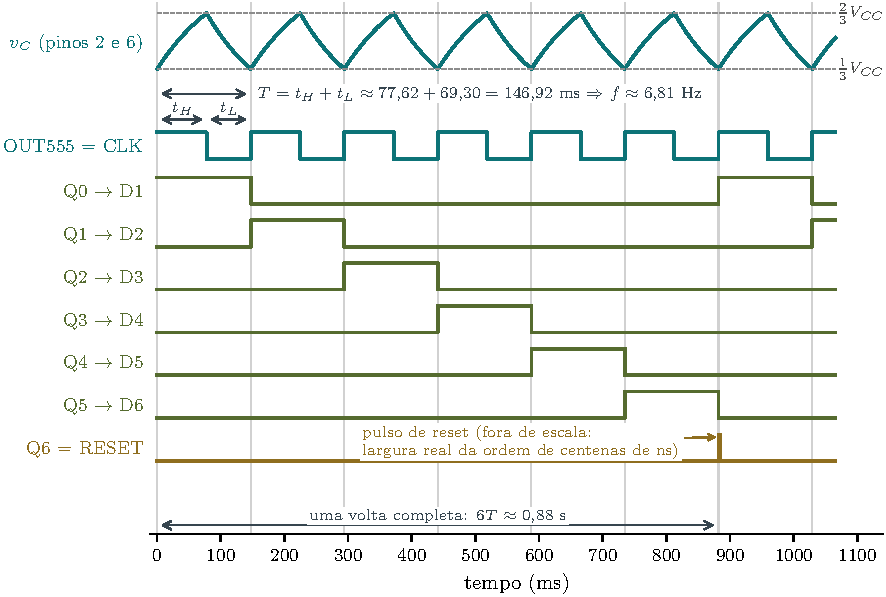
\includegraphics[width=\linewidth]{figuras/tempos-a4.pdf}
\caption{Diagrama de tempos ideal em regime permanente, calculado com R1, R2 e C2 do
esquemático. O pulso de reset está fora de escala.}
\end{figure}

\end{document}
